\documentclass[aspectratio=169,
  a4paper,uplatex,dvipdfmx,11pt,
  xcolor = {dvipsnames,svgnames},
  hyperref ={colorlinks=true,citecolor=Navy,linkcolor=NavyBlue,urlcolor=purple}
]{beamer}
\renewcommand{\baselinestretch}{1.4}

% ---refer `texdoc xcolor' at the command line---

% ---Display \subsubsection at the Index
% \setcounter{tocdepth}{3}

% ---Setting about the geometry of the document----
% \usepackage{a4wide}
% \pagestyle{empty}

% ---Physics and Math Packages---
\usepackage{amssymb,amsfonts,amsthm,mathtools}
\usepackage{physics,braket,bm}

% ---underline---
\usepackage{ulem}

% ---cancel---
\usepackage{cancel}

% --- surround the texts or equations
\usepackage{fancybox,ascmac}

% ---settings of theorem environment---
% \usepackage{amsthm}
% \theoremstyle{definition}

% ---settings of proof environment---
% \renewcommand{\proofname}{\textbf{証明}}
% \renewcommand{\qedsymbol}{$\blacksquare$}

% ---Ignore the Warnings---
\usepackage{silence}
\WarningFilter{latexfont}{Some font shapes,Font shape}
\ExplSyntaxOn
\msg_redirect_name:nnn{hooks}{generic-deprecated}{none}
\ExplSyntaxOff

% ---Insert the figure (If insert the `draft' at the option, the process becomes faster.)---
\usepackage{graphicx}
% \usepackage{subcaption}

% ----Add a link to a text---
\usepackage{url,hyperref}
\usepackage{xcolor}
\usepackage{pxjahyper}

% ---Tikz---
\usepackage{tikz,pgf,pgfplots,circuitikz}
\pgfplotsset{compat=1.15}
\usetikzlibrary{intersections,arrows.meta,angles,calc,3d,decorations.pathmorphing,positioning}

% ---Add the section number to the equation, figure, and table number---
\makeatletter
   \renewcommand{\theequation}{\thesection.\arabic{equation}}
   \@addtoreset{equation}{section}
   
   \renewcommand{\thefigure}{\thesection.\arabic{figure}}
   \@addtoreset{figure}{section}
   
   \renewcommand{\thetable}{\thesection.\arabic{table}}
   \@addtoreset{table}{section}
\makeatother

% ---enumerate---
% \renewcommand{\labelenumi}{$\arabic{enumi}.$}
% \renewcommand{\labelenumii}{$(\arabic{enumii})$}

% ---beamer settings---
\usefonttheme{professionalfonts}
% \usefonttheme{serif}
\usecolortheme{seahorse}
\setbeamercolor{structure}{fg=white}
\setbeamercolor{local structure}{fg=Turquoise}
\setbeamertemplate{itemize item}[ball]
\setbeamertemplate{enumerate item}[circle]
\setbeamercolor{bibliography entry author}{fg=black}
\setbeamercolor{bibliography item}{fg=black}
\setbeamercolor{alerted text}{fg=RoyalBlue}
\setbeamertemplate{frametitle continuation}{}
\setbeamertemplate{footline}[frame number]
\setbeamertemplate{navigation symbols}{} 

% ---tcolorbox---
\usepackage{tcolorbox}
\tcbuselibrary{raster,skins,theorems}
\newtcolorbox{bluebox}[2][]{enhanced,
colframe=RoyalBlue!40!white,
colback=RoyalBlue!10!white,
coltitle=black,
drop fuzzy shadow, title={#2}
,#1}
\newtcolorbox{blueboxblank}[1][]{enhanced,
colframe=RoyalBlue!40!white,
colback=RoyalBlue!10!white,
coltitle=black,
drop fuzzy shadow
,#1}
\newtcolorbox{redbox}[2][]{enhanced,
colframe=DarkRed!40!white,
colback=DarkRed!10!white,
coltitle=black,
drop fuzzy shadow, title={#2}
,#1}

% ---fonts---
\renewcommand{\familydefault}{\sfdefault}
\renewcommand{\kanjifamilydefault}{\gtdefault}
% \usepackage{newtxmath}
\mathversion{bold}

% ---citation---
\usepackage{usebib}
\newbibfield{author} 
\newbibfield{year} 
\newbibfield{journal} 
\newbibfield{doi} 
\bibinput{hoge}

\makeatletter
\newcommand*{\journal}{\begingroup\@makeother\#\@mylink}
\newcommand*{\@mylink}[1]{\href{http://dx.doi.org/\usebibentry{#1}{doi}}{\usebibentry{#1}{journal}}\endgroup} 
\makeatother

\newcommand*{\citefone}[2]{
  \begin{tikzpicture}[remember picture, overlay]
    \node[anchor=north east, align=left] at ($(current page.north east)-(0,0.0)$){
    {\tiny
      \cite{#1}
      #2,
      \journal{#1}
      (\usebibentry{#1}{year}).
    }
    };
  \end{tikzpicture}
}

\newcommand*{\citeftwo}[4]{
  \begin{tikzpicture}[remember picture, overlay]
    \node[anchor=north east, align=left] at ($(current page.north east)-(0,0.0)$){
    {\tiny
      \cite{#1}
      #2,
      \journal{#1}
      (\usebibentry{#1}{year}).
    }
    \\[-2.4ex]
    {\tiny
      \cite{#3}
      #4,
      \journal{#3}
      (\usebibentry{#3}{year}).
    }
    };
  \end{tikzpicture}
}

\newcommand*{\citefthree}[6]{
  \begin{tikzpicture}[remember picture, overlay]
    \node[anchor=north east, align=left] at ($(current page.north east)-(0,0.0)$){
    {\tiny
      \cite{#1}
      #2,
      \journal{#1}
      (\usebibentry{#1}{year}).
    }
    \\[-2.4ex]
    {\tiny
      \cite{#3}
      #4,
      \journal{#3}
      (\usebibentry{#3}{year}).
    }
    \\[-2.4ex]
    {\tiny
      \cite{#5}
      #6,
      \journal{#5}
      (\usebibentry{#5}{year}).
    }
    };
  \end{tikzpicture}
}

\newcommand*{\citefonev}[3]{
  \begin{tikzpicture}[remember picture, overlay]
    \node[anchor=north east, align=left, text width=#3cm] at ($(current page.north east)-(0,0.0)$){
    {{\fontsize{5pt}{0pt}\selectfont
      \cite{#1}
      #2,
      \journal{#1}
      (\usebibentry{#1}{year}).\par}
    }
    };
  \end{tikzpicture}
}

\newcommand*{\citeftwov}[5]{
  \begin{tikzpicture}[remember picture, overlay]
    \node[anchor=north east, align=left, text width=#5cm] at ($(current page.north east)-(0,0.0)$){
    {{\fontsize{5pt}{0pt}\selectfont
      \cite{#1}
      #2,
      \journal{#1}
      (\usebibentry{#1}{year}).\par}

      {\fontsize{5pt}{0pt}\selectfont
      \cite{#3}
      #4,
      \journal{#3}
      (\usebibentry{#3}{year}).\par}
    }
    };
  \end{tikzpicture}
}

\newcommand*{\citefthreev}[7]{
  \begin{tikzpicture}[remember picture, overlay]
    \node[anchor=north east, align=left, text width=#7cm] at ($(current page.north east)-(0,0.0)$){
    {{\fontsize{5pt}{0pt}\selectfont
    \cite{#1}
    #2,
    \journal{#1}
    (\usebibentry{#1}{year}).\par}

    {\fontsize{5pt}{0pt}\selectfont
    \cite{#3}
    #4,
    \journal{#3}
    (\usebibentry{#3}{year}).\par}

    {\fontsize{5pt}{0pt}\selectfont
    \cite{#5}
    #6,
    \journal{#5}
    (\usebibentry{#5}{year}).\par}
    }
    };
  \end{tikzpicture}
}


% ---Title---
\title{
  卒業研究
  \texorpdfstring{\\}{}
  \texorpdfstring{\vspace*{5pt}}{}
  {\LARGE
    磁化トーラス上にコンパクト化した
    \\
    超対称模型におけるモジュライ固定
  }
}
\author{
  安倍研究室 \ B4
  \texorpdfstring{\\}{}
  \texorpdfstring{\vspace*{3pt}}{}
  宮根 一樹
}
\date{2024年2月5日(月)}



\begin{document}

\begin{frame}
  \titlepage
\end{frame}


\section{イントロダクション}

\begin{frame}
  \frametitle{\thesection.\ \secname}
  \begin{columns}[t]    
    \begin{column}{0.4\textwidth} 
      素粒子標準模型
      \begin{itemize}
        \item
        実験により高い精度で検証
        \item 
        物質場は3世代・左右非対称
      \end{itemize}
      \vspace*{-5pt}
      \begin{center}
        $\downarrow$
      \end{center}
      \vspace*{-5pt}
      標準模型の問題点
      \begin{itemize}
        \item 
        量子重力が含まれていない
        \item 
        世代間の質量階層性
      \end{itemize}
      など    
    \end{column}
    \begin{column}{0.4\textwidth}  

      \vspace*{-1.2cm}

      $\longrightarrow$高次元時空モデルの考案    
      \begin{itemize}
        \item[\textcolor{black}{\uline{e.g.}}]    
        超弦理論    
        \item 
        量子重力を含む
        \item 
        \uline{10次元}で無矛盾な理論
      \end{itemize}      
      \vspace*{-5pt}
      \begin{center}
        $\downarrow$
      \end{center}
      \vspace*{-5pt}
      現実的な模型を得るためには
      \begin{itemize}
        \item 
        余剰空間を\textcolor{red}{観測と矛盾のないように小さくコンパクト化}
        \item 
        素粒子標準模型の世代数,\ \ 質量や結合定数などを再現
      \end{itemize}
    \end{column}
  \end{columns}
  \begin{tikzpicture}[remember picture, overlay]
    \draw[thin] (7.5,0.2)--(7.5,8);
  \end{tikzpicture}
\end{frame}

\begin{frame}
  \frametitle{\thesection.\ \secname}
  \citefone{Abe_PhenomenologicalAspects_2013}{H. Abe, T. Kobayashi, H. Ohki, A. Oikawa, and K. Sumita}

  \vspace*{-1.1cm}

  余剰空間と4次元有効理論の関係

  \vspace*{5pt}

  \uline{e.g.}
  {\small
  \quad
  $\displaystyle
    \int\dd^{10}X
    \sqrt{-G}\frac{1}{g^2}\text{Tr}\left[ -\frac{1}{4}F^{MN}F_{MN} \right]
    \rightarrow
    \int\dd^{4}x
    \underbrace{
      \left(  
        \textcolor{DarkRed}{
        \int\dd^{6}y
        \sqrt{-G}\frac{1}{g^2}
        }
      \right)
    }_{=\dfrac{1}{g_{\text{4D}}^2}}
    \text{Tr}\left[ -\frac{1}{4}F^{\mu\nu}F_{\mu\nu} \right]
  $
  }

  \begin{center}
    \doublebox{余剰空間の幾何は4次元有効理論の結合定数を決定する}
  \end{center}

  \hspace*{1cm}時空の計量は力学的な場

  \vspace*{-5pt}

  \begin{center}
    $\displaystyle
      \dd s^{10}
      =
      \textcolor{RoyalBlue}{g_{\mu\nu}(x,y)}\dd x^{\mu}\dd x^{\nu}
      +
      \textcolor{RoyalBlue}{g_{mn}(x,y)}\dd y^{m}\dd y^{n}
    $      
  \end{center}

  $\rightarrow$
  真空期待値$\ev*{g_{mn}}$は\textcolor{red}{$g_{mn}(x,y)$の力学(ポテンシャル)で決定される}

\end{frame}

\begin{frame}
  \frametitle{\thesection.\ \secname}
  \citeftwo{Abe_SuperfieldDescription_2012}{H. Abe, T. Kobayashi, H. Ohki, and K. Sumita}{Abe_AhlerModuli_2017}{H. Abe, T. Kobayashi, K. Sumita, and S. Uemura}

  \vspace*{-30pt}

  \begin{columns}[t]    
    \begin{column}{0.65\textwidth} 
      \begin{itemize}
        \item 
        余剰空間の計量$g_{mn}(x)$:
        \\
        4次元有効理論ではスカラー場(\textcolor{DarkRed}{モジュライ})
        \item 
        ポテンシャルの(準)安定点でモジュライが
        \\
        真空期待値を獲得(\textcolor{DarkRed}{モジュライ固定})
      \end{itemize}
    \end{column}
    \begin{column}{0.35\textwidth} 
      \vspace*{0.2cm}

      \centering
      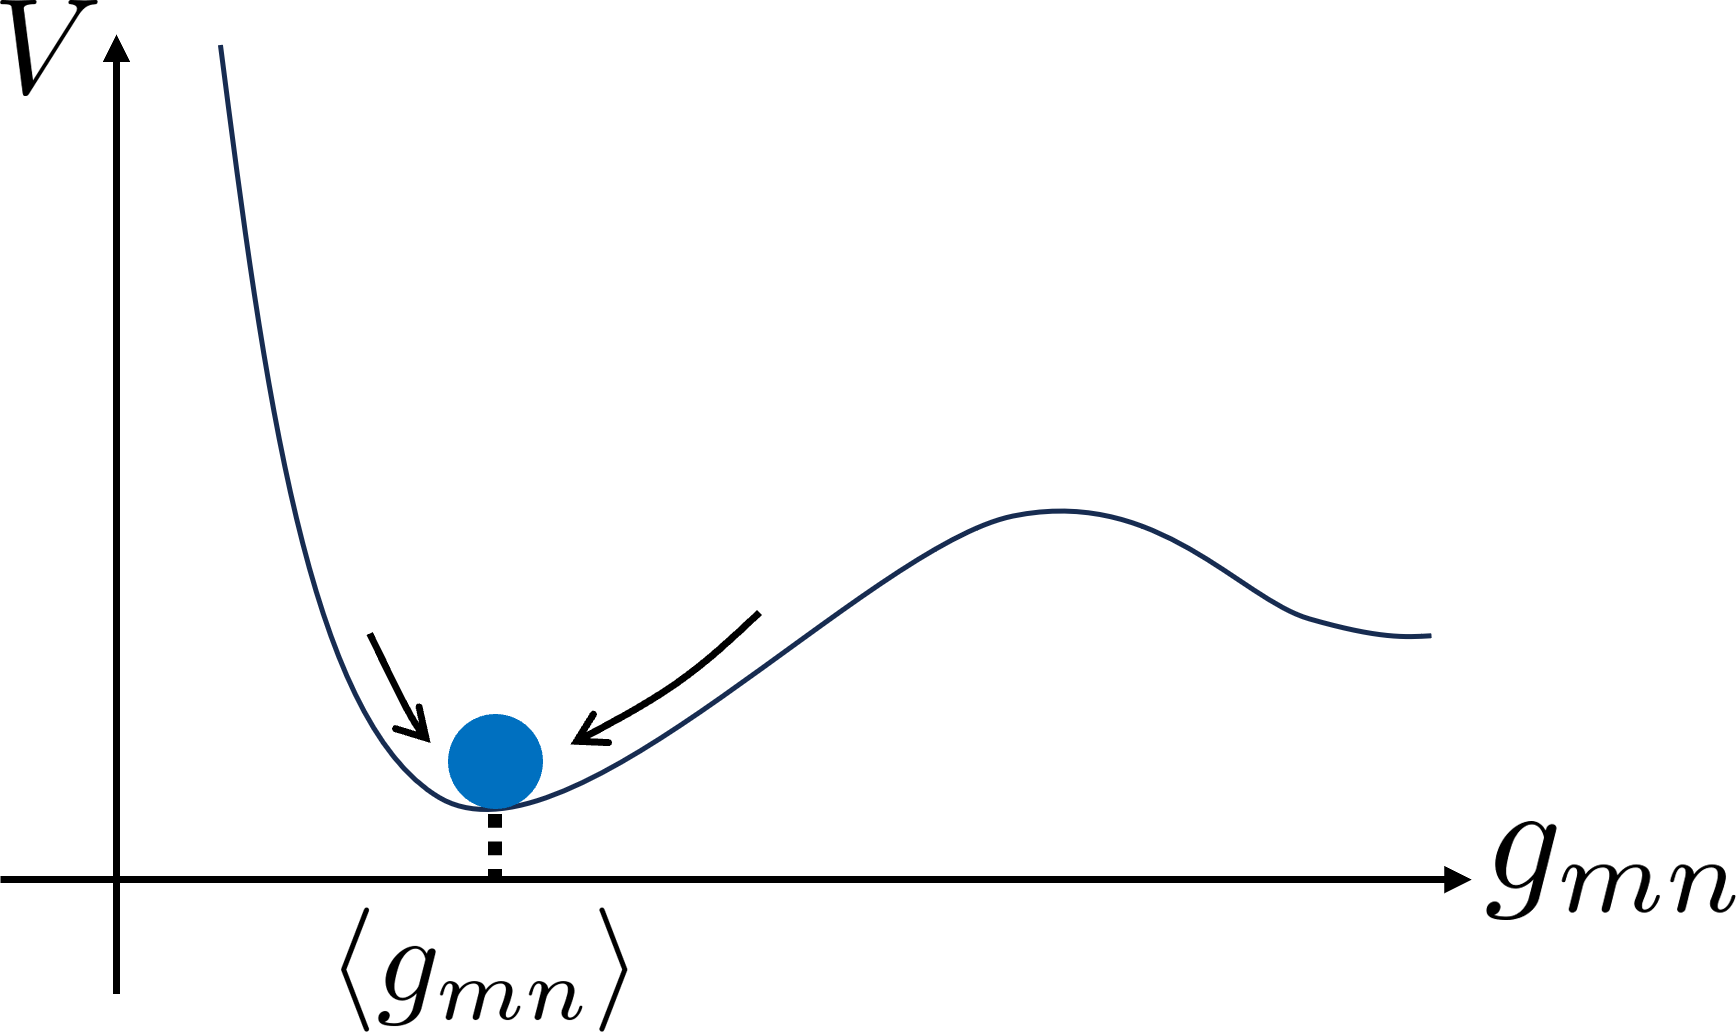
\includegraphics[width=1.0\textwidth]{fig/vev_idea.png}
    \end{column}
  \end{columns}

  \pause

  \begin{center}
    {\Large $\downarrow$}
  \end{center}

  \begin{bluebox}{本研究の目的}
    標準模型の世代構造を再現する磁化トーラス模型\cite{Abe_SuperfieldDescription_2012,Abe_AhlerModuli_2017}のモジュライ固定

    \vspace*{-5pt}

    \begin{flushright}
      $\rightarrow$
      余剰空間の大きさが観測と整合するか?
    \end{flushright}
  \end{bluebox}

\end{frame}

\section{磁化トーラス模型}

\begin{frame}
  \frametitle{\thesection.\ \secname}
  \citeftwo{Abe_SuperfieldDescription_2012}{H. Abe, T. Kobayashi, H. Ohki, and K. Sumita}{Cremades_ComputingYukawa_2004a}{D. Cremades, L. E. Ibanez, and F. Marchesano}

  \vspace*{-20pt}

  \uline{トーラスコンパクト化}
  \begin{itemize}
    \item 
    6次元余剰空間$\rightarrow$\uwave{3つのトーラス$T^{2}$}にコンパクト化
    \\
    \vspace*{5pt}
    \hspace*{2.8cm}
\includegraphics[width=0.4\textwidth]{fig/torus/tori.png}
    \\
    \hspace*{3.0cm}
    $\mathcal{A}^{(1)}$
    \hspace*{1.0cm}
    $\mathcal{A}^{(2)}$
    \hspace*{1.0cm}
    $\mathcal{A}^{(3)}$
    \hspace*{0.5cm}
    $\longleftarrow$トーラスの面積
    \item 
    $\mathcal{A}^{(i)}(x)$は\textcolor{DarkMagenta}{モジュライ}
  \end{itemize}

  \begin{columns}[t]    
    \begin{column}{0.5\textwidth} 
      \uline{磁束}
      \begin{itemize}
        \item 
        トーラス上の2種のゲージ場に
        \vspace*{-5pt}
        \begin{flushright}
          それぞれ磁場$M_{a}^{(i)}$を導入    
          \\     
          $(a=1,2)$      
        \end{flushright}
      \end{itemize}
    \end{column}
    \begin{column}{0.48\textwidth} 
      \vspace*{-15pt}
      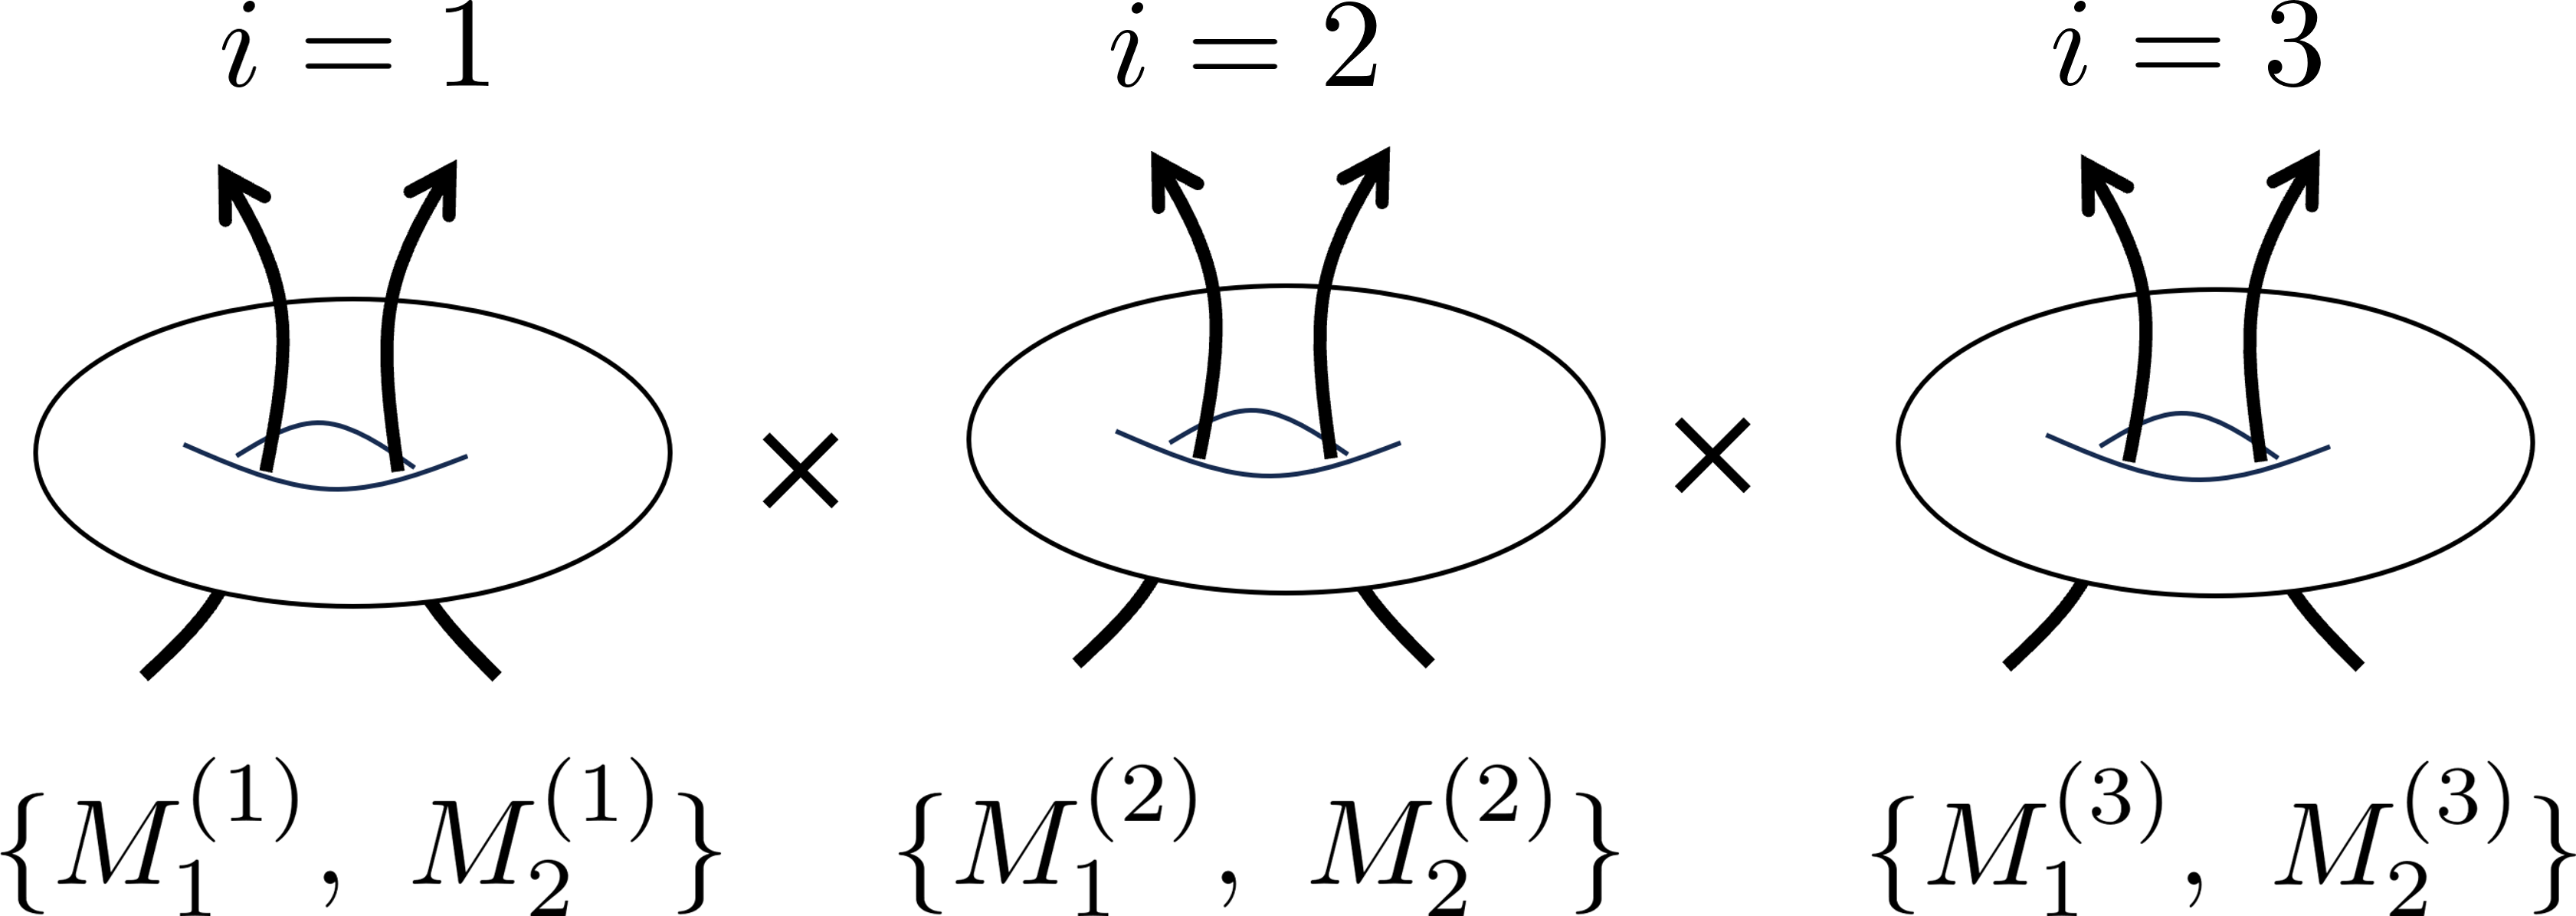
\includegraphics[width=1.0\textwidth]{fig/torus/tori_fluxed.png}
    \end{column}
  \end{columns}

\end{frame}

\begin{frame}
  \frametitle{\thesection.\ \secname}

  \begin{bluebox}{\empty}
    \centering
    磁場ポテンシャルによる面積比の固定
  \end{bluebox}

  \uline{磁場のポテンシャル}\qquad 
  $
    F^{MN}F_{MN}
    =
    F^{\mu\nu}F_{\mu\nu}
    +
    \uwave{F^{mn}F_{mn}}
    +
    \cdots
  $
  \\
  \hspace*{9cm}{\Large $\downarrow$}
  \begin{equation}
    V^{(D)}
    =
    \pi^2
    \prod_{i}\mathcal{A}^{i}
    \times
    \left\{
      \uline{
      \left(  
        \sum_{i}\frac{M_{1}^{(i)}}{\mathcal{A}^{(i)}}
      \right)^2
      }
      +
      \uline{
      \left( 
        \sum_{i}\frac{M_{2}^{(i)}}{\mathcal{A}^{(i)}}
      \right)^2
      }
    \right\}
    \nonumber
  \end{equation}
  \hspace*{6.2cm}
  それぞれがゼロのときに$\ev*{V^{(D)}}=0$\ (最小)

  \begin{center}
    \tikz[baseline=(x.base)]{
      \node(x)[rectangle, fill=DarkRed!10, rounded corners]{
        \ 
        $
        \displaystyle
        \frac{M_{a}^{(1)}}{\ev*{\mathcal{A}^{(1)}}}
        +
        \frac{M_{a}^{(2)}}{\ev*{\mathcal{A}^{(2)}}}
        +
        \frac{M_{a}^{(3)}}{\ev*{\mathcal{A}^{(3)}}}
        =
        0
        \quad
        \text{for}
        \ 
        a=1,2$\ };
    }    
  \end{center}

\end{frame}


\begin{frame}
  \frametitle{\thesection.\ \secname}

  \vspace*{-10pt}

  \uline{真空期待値$\ev*{\mathcal{A}^{(1)}},\ev*{\mathcal{A}^{(2)}},\ev*{\mathcal{A}^{(3)}}$の関係}
  \begin{gather}
    M_{a}^{(1)}
    +
    M_{a}^{(2)}
    \frac{\ev*{\mathcal{A}^{(1)}}}{\ev*{\mathcal{A}^{(2)}}}
    +
    M_{a}^{(3)}
    \frac{\ev*{\mathcal{A}^{(1)}}}{\ev*{\mathcal{A}^{(3)}}}
    =
    0
    \quad
    \text{for}
    \ 
    a=1,2
    \nonumber    
    \\
    \text{\Large $\downarrow$}
    \nonumber
    \\
    \hspace*{-10pt}
    \frac{\ev*{\mathcal{A}^{(1)}}}{\ev*{\mathcal{A}^{(2)}}}
    =
    \frac{
      M_{1}^{(3)} M_{2}^{(1)}-M_{1}^{(1)} M_{2}^{(3)}
    }{
      M_{1}^{(2)} M_{2}^{(3)}- M_{1}^{(3)} M_{2}^{(2)}
    }
    \ ,\ 
    \frac{\ev*{\mathcal{A}^{(1)}}}{\ev*{\mathcal{A}^{(3)}}}
    =
    -\frac{
      M_{1}^{(2)} M_{2}^{(1)}-M_{1}^{(1)} M_{2}^{(2)}
    }{
      M_{1}^{(2)} M_{2}^{(3)}-M_{1}^{(3)} M_{2}^{(2)}
    }
    \nonumber
  \end{gather}
  \begin{center}
    \doublebox{面積の比は磁場のポテンシャルによって決定された}
  \end{center}
  \pause
  \begin{redbox}{\empty}
    \centering
    全体の因子は不定
    $\longrightarrow$
    磁場とは異なる起源をもつポテンシャルを導入する
  \end{redbox}
\end{frame}


\section{全体の因子の決定}

\begin{frame}
  \frametitle{\thesection.\ \secname}
  \begin{tikzpicture}[remember picture, overlay]
    \node[anchor=north east, align=left] at ($(current page.north east)-(0,0.0)$){
      {\tiny
        \cite{Wess_SupersymmetrySupergravity_1992} J. Wess and J. Bagger, 1992.
      }
    \\[-2.4ex]
    {\tiny
      \cite{Abe_ModuliStabilization_2007a}
      H. Abe, T. Higaki, T. Kobayashi, and Y. Omura,
      \journal{Abe_ModuliStabilization_2007a}
      (\usebibentry{Abe_ModuliStabilization_2007a}{year}).
    }
    };
  \end{tikzpicture}

  \vspace*{-20pt}

  全体の因子を決定するモジュライ:$T$
  \qquad
  $\longleftarrow\ev*{\mathcal{A}^{(1)}},\ev*{\mathcal{A}^{(2)}},\ev*{\mathcal{A}^{(3)}}\propto\ev*{T}$

  \vspace{10pt}

  \uline{$T$の有効ポテンシャル}
  \begin{itemize}
    \item 
    有効理論は超対称性(ボゾンとフェルミオンの対称性)をもつ
    \item 
    超対称作用はスーパーポテンシャル$W$とケーラーポテンシャル$K$で決定\cite{Wess_SupersymmetrySupergravity_1992}
    \item 
    本研究では以下のポテンシャルを用いる\cite{Abe_ModuliStabilization_2007a}:

    \vspace*{-15pt}
  
    \begin{equation}
      \left\{
        \begin{alignedat}{1}
          W
          &=
          w_{0}-Ae^{-a\textcolor{DarkRed}{T}}+B\textcolor{DarkBlue}{X}
          \\
          K
          &=
          -
          \ln (\textcolor{DarkRed}{T}+\textcolor{DarkRed}{\bar{T}})
          +
          \textcolor{DarkBlue}{|X|^2}
        \end{alignedat}
      \right.
      \nonumber
    \end{equation}
    \begin{center}
      \small
      $\textcolor{DarkBlue}{X}$は新たに導入したスカラー場
      ,
      $w_{0}, A, B, a$は実パラメター      
    \end{center}
  \end{itemize}

\end{frame}

\section{結果}

\begin{frame}
  \frametitle{\thesection.\ \secname}
  \citefone{Abe_ModuliStabilization_2007a}{H. Abe, T. Higaki, T. Kobayashi, and Y. Omura}

  \vspace*{-20pt}

  {\small
  プランクスケール$M_{\text{Pl}}(\sim 2.4\times 10^{18}\ \text{GeV})=1$の単位系
  }

  \begin{columns}[t]    
    \begin{column}{0.6\textwidth} 
      \uline{スカラーポテンシャル}
      \vspace*{-5pt}
      \begin{gather}
        V^{(F)}
        =
        e^{K}(K^{I\bar{J}}(D_{I}W)(D_{\bar{J}}\bar{W})-3|W|^2)
        \nonumber
        \\
        \left\{
          \begin{alignedat}{1}
            D_{I}W
            &\equiv
            \partial_{I}W+(\partial_{I}K)W
            \\
            K^{I\bar{J}}
            &\text{:$\partial_{I}\partial_{\bar{J}}K$の逆行列}        
          \end{alignedat}
        \right.
        \quad
        (I=X,T)
        \nonumber
      \end{gather}
    \end{column}
    \begin{column}{0.38\textwidth} 
      \vspace*{-5pt}
      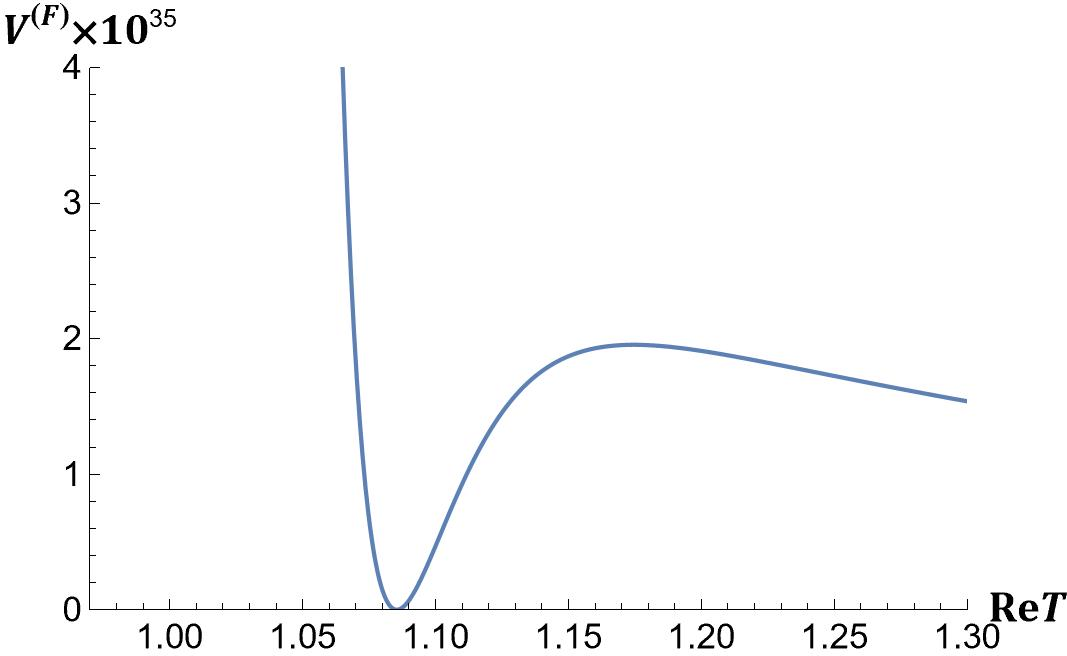
\includegraphics[width=1.0\textwidth]{fig/aaaa.jpg}
    \end{column}
  \end{columns}

  \vspace*{10pt}

  パラメター:
    $
    w_{0}
    \sim
    2.17
    \times
    10^{-18}
    \ ,\ 
    a=4\pi^2
    \ ,\ 
    A=1
    \ ,\ 
    B=e^{-4\pi^2}
    $
  \begin{center}
    $\rightarrow \ev*{T}\sim 1.085$に固定
  \end{center}

  \begin{tikzpicture}[remember picture, overlay]
    \node[anchor=north east, align=left] at ($(current page.north east)-(0,0.7)$){
    {      
      \small
      \tikz[baseline=(x.base)]{
        \node(x)[rectangle, fill=blue!10, rounded corners]{
          $W
          =
          w_{0}-Ae^{-a\textcolor{DarkRed}{T}}+B\textcolor{DarkBlue}{X}
          \ ,\ 
          K
          =
          -
          \ln (\textcolor{DarkRed}{T}+\textcolor{DarkRed}{\bar{T}})
          +
          \textcolor{DarkBlue}{|X|^2}$};
      }
    }
    };
  \end{tikzpicture}

\end{frame}

\begin{frame}
  \frametitle{\thesection.\ \secname}
  \begin{tikzpicture}[remember picture, overlay]
    \node[anchor=north east, align=left] at ($(current page.north east)-(0,0.0)$){
    {\tiny
      \cite{Abe_AhlerModuli_2017}
      H. Abe, T. Kobayashi, K. Sumita, and S. Uemura,
      \journal{Abe_AhlerModuli_2017}
      (\usebibentry{Abe_AhlerModuli_2017}{year}).
    }
    \\[-2.4ex]
    {\tiny
    [7]

    R.L. Workmanet al.(Particle Data Group), Prog.Theor.Exp.Phys.2022, 083C01 (2022) and 2023 update.
    }
    };
  \end{tikzpicture}

  \vspace*{-20pt}

  磁場の値は先行研究\cite{Abe_AhlerModuli_2017}の値
  \qquad
  $\longleftarrow$標準模型の世代構造を再現
  \begin{center}
    \small
    $
      \{M_{1}^{(1)},M_{2}^{(1)}\}
      =
      \{7,-7\}
      \ ,\ 
      \{M_{1}^{(2)},M_{2}^{(2)}\}
      =
      \{1,0\}
      \ ,\ 
      \{M_{1}^{(3)},M_{2}^{(3)}\}
      =
      \{0,-1\}        
    $
  \end{center}

  \begin{center}      
    面積比\quad
    \tikz[baseline=(x.base)]{
      \node(x)[rectangle, fill=DarkRed!10, rounded corners]{
        \        
    $\displaystyle
    \frac{\mathcal{A}^{(2)}}{\mathcal{A}^{(1)}}
    =
    \frac{\mathcal{A}^{(3)}}{\mathcal{A}^{(1)}}
    =
    \frac{1}{7}    
    $\ };
    }    
    \qquad\quad
    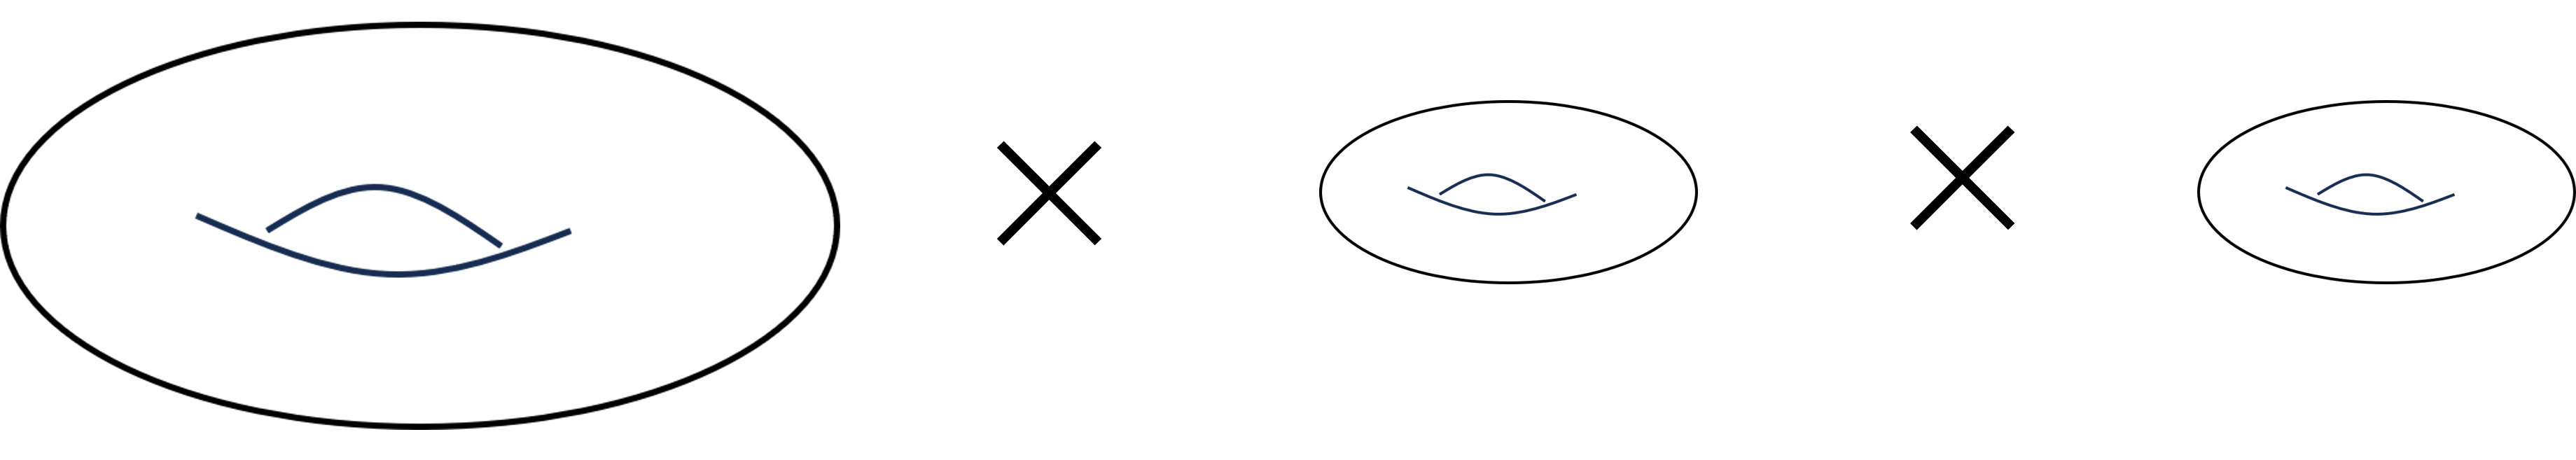
\includegraphics[width=0.55\textwidth]{fig/torus/result_ori.png}
  \end{center}

  \vspace*{-10pt}

  \begin{center}
    \hspace*{-24pt}
    \begin{tabular}{rl|cl}
      & 
      第1トーラスの面積 & 実験による制限(参考[7]) & \\
      $\ev*{\mathcal{A}^{(1)}}$ & $\sim (10^{-35}\ \text{m})^2$ & $R_{6\text{D}}<\mathcal{O}(10^{-6}\ \text{m})$ & (6次元万有引力への制限)
      \\
      & $\sim (10^{19}\ \text{GeV})^{-2}$ & $M_{\text{KK}}>\mathcal{O}(10^{3}\ \text{GeV})$ & (KK粒子生成の制限)
    \end{tabular}
  \end{center}

\end{frame}


% --------------------------

\section{まとめ・展望}

\begin{frame}
  \frametitle{\thesection.\ \secname}

  \uline{まとめ}
  \begin{itemize}
    \item 
    磁化トーラス模型におけるモジュライ(トーラスの面積)の固定を議論
    \item 
    面積比は磁場のポテンシャル$V^{(D)}$のみで決定(ただし,全体の因子は不定)
    \item 
    磁場とは異なる起源をもつポテンシャル$V^{(F)}$により全体の因子を決定
  \end{itemize}

  \uline{展望}
  \begin{itemize}
    \item 
    より一般的なポテンシャル$V^{(F)}$によるモジュライ固定
    \item 
    超対称性の自発的破れ,超対称粒子の質量などについて議論
  \end{itemize}

\end{frame}

% --------------------------

\newcounter{Appendix}
\setcounter{Appendix}{\value{framenumber}}
\setcounter{section}{0}
\renewcommand{\thesubsection}{\Alph{subsection}}
\makeatletter
   \renewcommand{\theequation}{\thesubsection.\arabic{equation}}
   \@addtoreset{equation}{section}
   
   \renewcommand{\thefigure}{\thesubsection.\arabic{figure}}
   \@addtoreset{figure}{section}
   
   \renewcommand{\thetable}{\thesubsection.\arabic{table}}
   \@addtoreset{table}{section}
\makeatother

\section{付録}

\begin{frame}[plain]
  \frametitle{\ }
  \huge \secname
\end{frame}

\subsection{背景磁場}

\begin{frame}[plain]
  \frametitle{\thesubsection.\ \subsecname}
  \citefone{Abe_SuperfieldDescription_2012}{H. Abe, T. Kobayashi, H. Ohki, and K. Sumita}

  \vspace*{-10pt}

  真空期待値を次のように決定
  \begin{equation}
    \ev*{A_{i}}
    =
    \frac{\pi}{\Im \tau_{i}}\textcolor{black}{M^{(i)}}\bar{z}_{i}
    \ ,\quad
    \textcolor{black}{
      M^{(i)}
    }
    \textcolor{black}{
      =
      \begin{pmatrix}
        M_{1}^{(i)} &0 &\cdots & 0\\
        0&M_{2}^{(i)}&\cdots&0\\
        \vdots& \vdots& \ddots &\vdots \\
        0 & 0 & \cdots & M_{N}^{(i)}
      \end{pmatrix}
    }
    \nonumber
  \end{equation}

  \begin{itemize}
    \color{black}
    \item 
    $M_{a}^{(i)}$は整数
    \item 
    $M^{(i)}$はトーラス上の磁場
    $\rightarrow$
    $F_{45}=\pi M^{(1)}$など
    \item 
    ブロック対角化でより小さいゲージ対称性

    \vspace*{-20pt}

    $$
      U(N)
      \rightarrow
      U(N_1)
      \times
      U(N_2)
      \times
      \cdots
      \times
      U(\tilde{N})
    $$
  \end{itemize}
  
\end{frame}


\subsection{\texorpdfstring{$F$}{F}-term uplifting}

\begin{frame}[plain]
  \frametitle{\thesubsection.\ \subsecname}


  \begin{columns}[t]    
    \begin{column}{0.5\textwidth} 
      \centering
      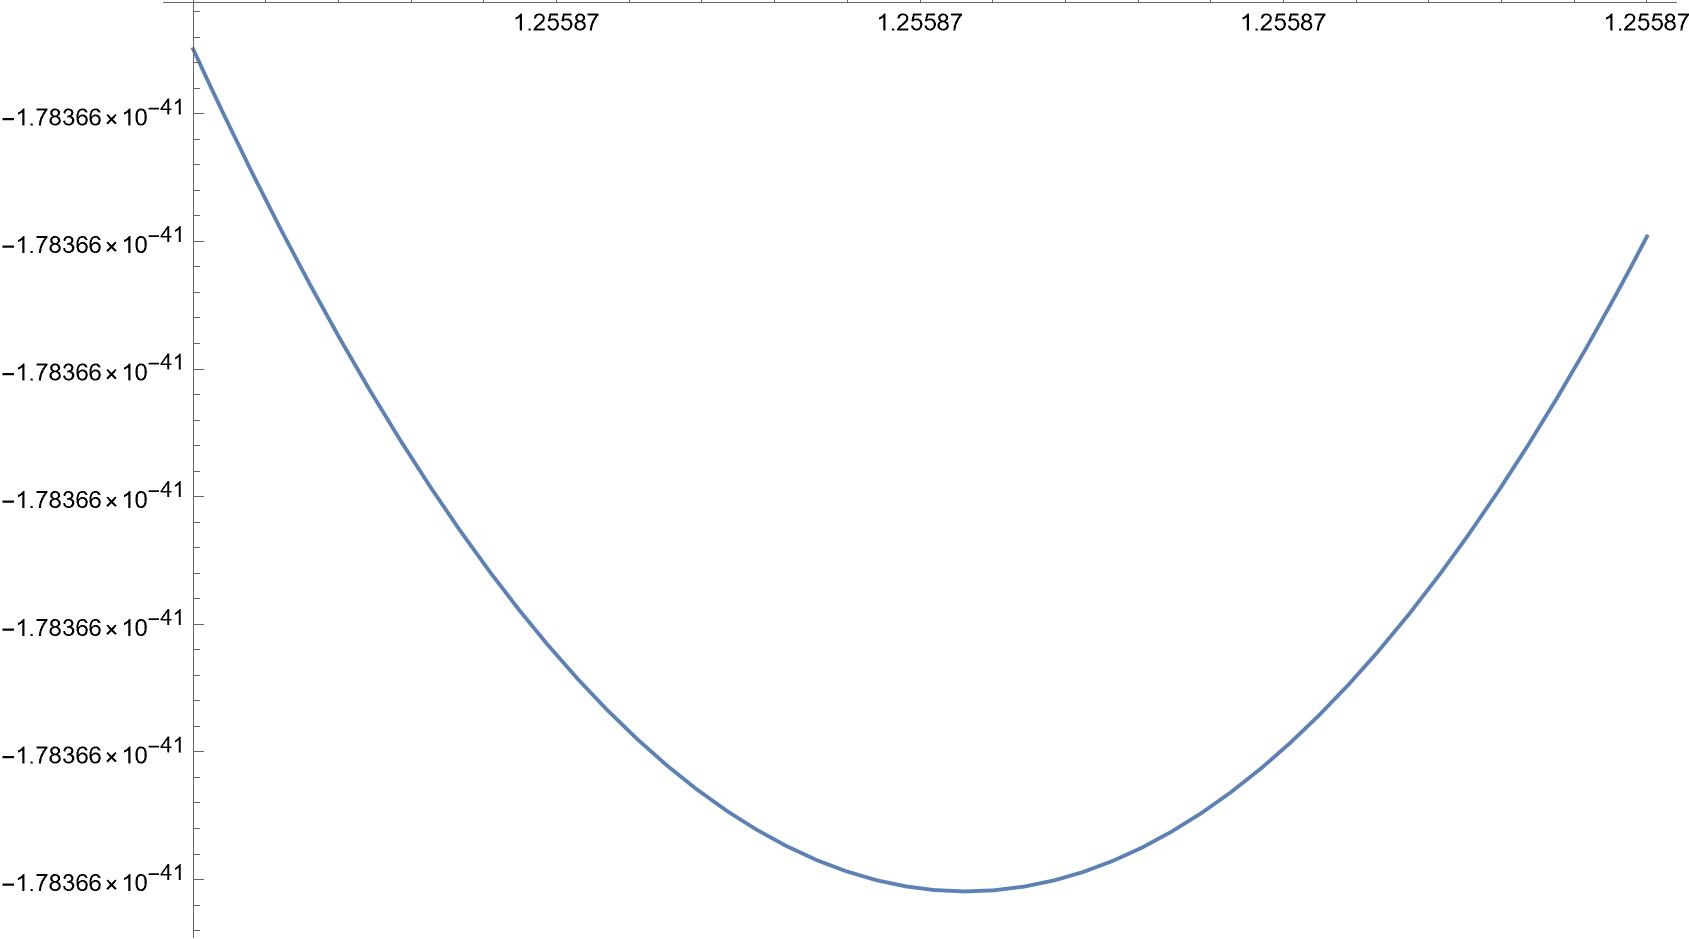
\includegraphics[width=1.0\textwidth]{fig/kklt_minimum.jpg}  
      \begin{equation}
        \left\{
          \begin{alignedat}{1}
            W
            &=
            w_{0}-Ae^{-a\textcolor{DarkRed}{T}}
            \\
            K
            &=
            -
            \ln (\textcolor{DarkRed}{T}+\textcolor{DarkRed}{\bar{T}})
          \end{alignedat}
        \right.
        \nonumber
      \end{equation}
    \end{column}
    \begin{column}{0.5\textwidth} 
      \centering
      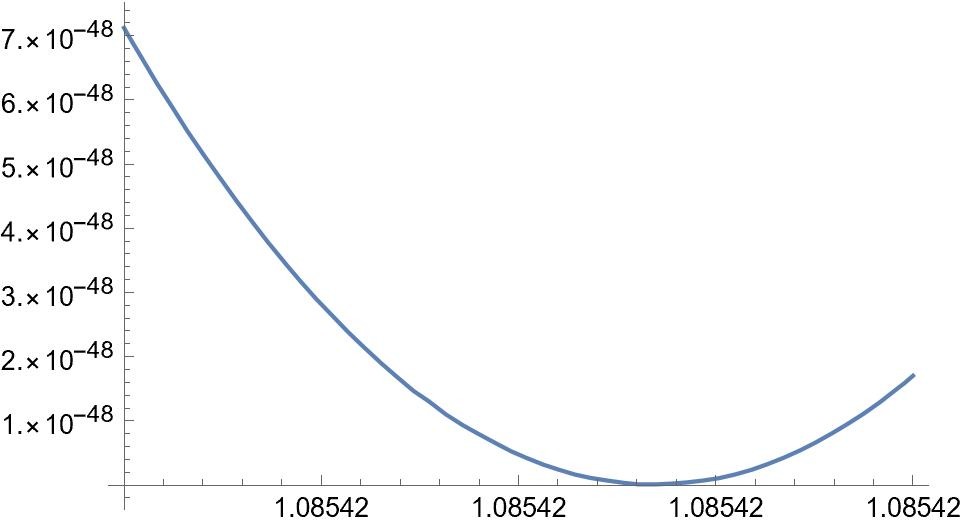
\includegraphics[width=1.0\textwidth]{fig/polonyi_kklt_minimum.jpg}  
      \begin{equation}
        \left\{
          \begin{alignedat}{1}
            W
            &=
            w_{0}-Ae^{-a\textcolor{DarkRed}{T}}+B\textcolor{DarkBlue}{X}
            \\
            K
            &=
            -
            \ln (\textcolor{DarkRed}{T}+\textcolor{DarkRed}{\bar{T}})
            +
            \textcolor{DarkBlue}{|X|^2}
          \end{alignedat}
        \right.
        \nonumber
      \end{equation}
    \end{column}
  \end{columns}
  
\end{frame}


% \begin{frame}[plain]
%   \frametitle{\thesubsection\ \subsecname}







  
% \end{frame}

% --------------------------

\section{参考文献}
\begin{frame}[plain,allowframebreaks]
  \frametitle{\secname}
  \scriptsize
  \beamertemplatetextbibitems
  \bibliographystyle{ytphys}
  \bibliography{hoge}
\end{frame}


\setcounter{framenumber}{\value{Appendix}}
\end{document}
